\documentclass[tikz,border=4pt]{standalone}
% Shared style for MultiMM figures (white background, logo palette)
\usepackage{tikz,pgfplots,amsmath}
\pgfplotsset{compat=1.16}
\usetikzlibrary{arrows.meta,calc,decorations.pathreplacing,positioning,backgrounds}
\definecolor{indigo}{HTML}{3B37A0}
\definecolor{violet}{HTML}{6A3AA8}
\definecolor{crimson}{HTML}{B5406C}
\definecolor{gold}{HTML}{E9A62C}
\definecolor{golddark}{HTML}{B9791A}
\definecolor{grey}{HTML}{8A8AA0}
\definecolor{lightgrey}{HTML}{E4E4EE}
\tikzset{
  bead/.style={circle,draw=#1!80!black,fill=#1!35,line width=0.5pt,minimum size=9pt,inner sep=0pt},
  bead/.default=indigo,
  lab/.style={font=\small},
}
\pgfplotsset{
  every axis/.append style={
    width=9.5cm,height=6.3cm,axis lines=left,line width=0.5pt,
    grid=major,grid style={draw=lightgrey,line width=0.3pt},
    tick label style={font=\small},label style={font=\normalsize},
    legend style={font=\footnotesize,draw=none,fill=white,fill opacity=0.8,text opacity=1},
    legend cell align=left,
  },
  every axis plot/.append style={line width=1.2pt,smooth},
}

\begin{document}
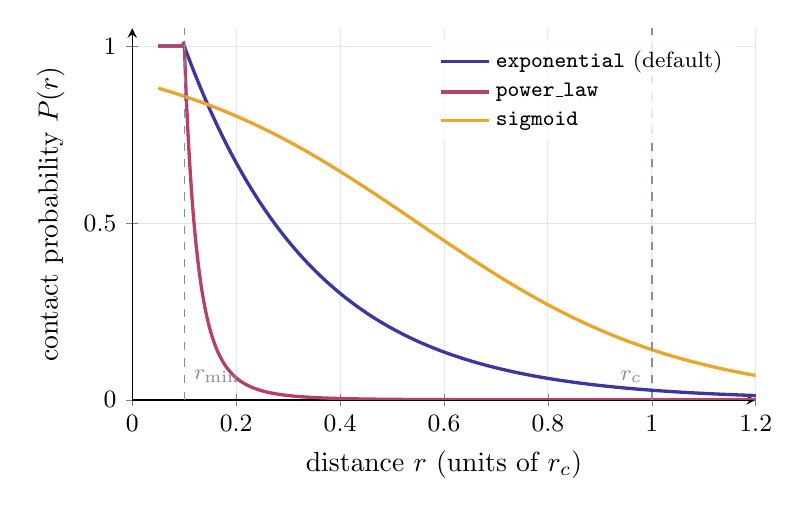
\begin{tikzpicture}
\begin{axis}[xlabel={distance $r$ (units of $r_c$)},ylabel={contact probability $P(r)$},
  xmin=0,xmax=1.2,ymin=0,ymax=1.05,legend pos=north east,domain=0.05:1.2,samples=300]
\addplot[indigo] {min(1,exp(-(x-0.1)/0.25))};
\addlegendentry{\texttt{exponential} (default)}
\addplot[crimson] {min(1,(0.1/x)^4)};
\addlegendentry{\texttt{power\_law}}
\addplot[gold] {1/(1+exp(4*(x-0.55)))};
\addlegendentry{\texttt{sigmoid}}
\draw[dashed,grey] (axis cs:0.1,0) -- (axis cs:0.1,1.05);
\node[font=\footnotesize,grey,anchor=south west] at (axis cs:0.1,0.02) {$r_{\min}$};
\draw[dashed,grey] (axis cs:1,0) -- (axis cs:1,1.05);
\node[font=\footnotesize,grey,anchor=south east] at (axis cs:1,0.02) {$r_c$};
\end{axis}
\end{tikzpicture}
\end{document}
